\section*{Energy Calibration}

Before proceeding to study the branching ratio each detector have to be energy calibrated. In order to do so, a $^{22}$Na source was used due to the fact that, NaI(Tl) scintillators, are sensible to photopeak so is possible to use the 511 and  1275 keV photopeak of the sodium source for the purpose of rescaling energy spectra. Calibrated spectrum for each detector is presented in Fig.~\ref{Fig: calibrated spectra}.

\begin{figure}[H]
\centering
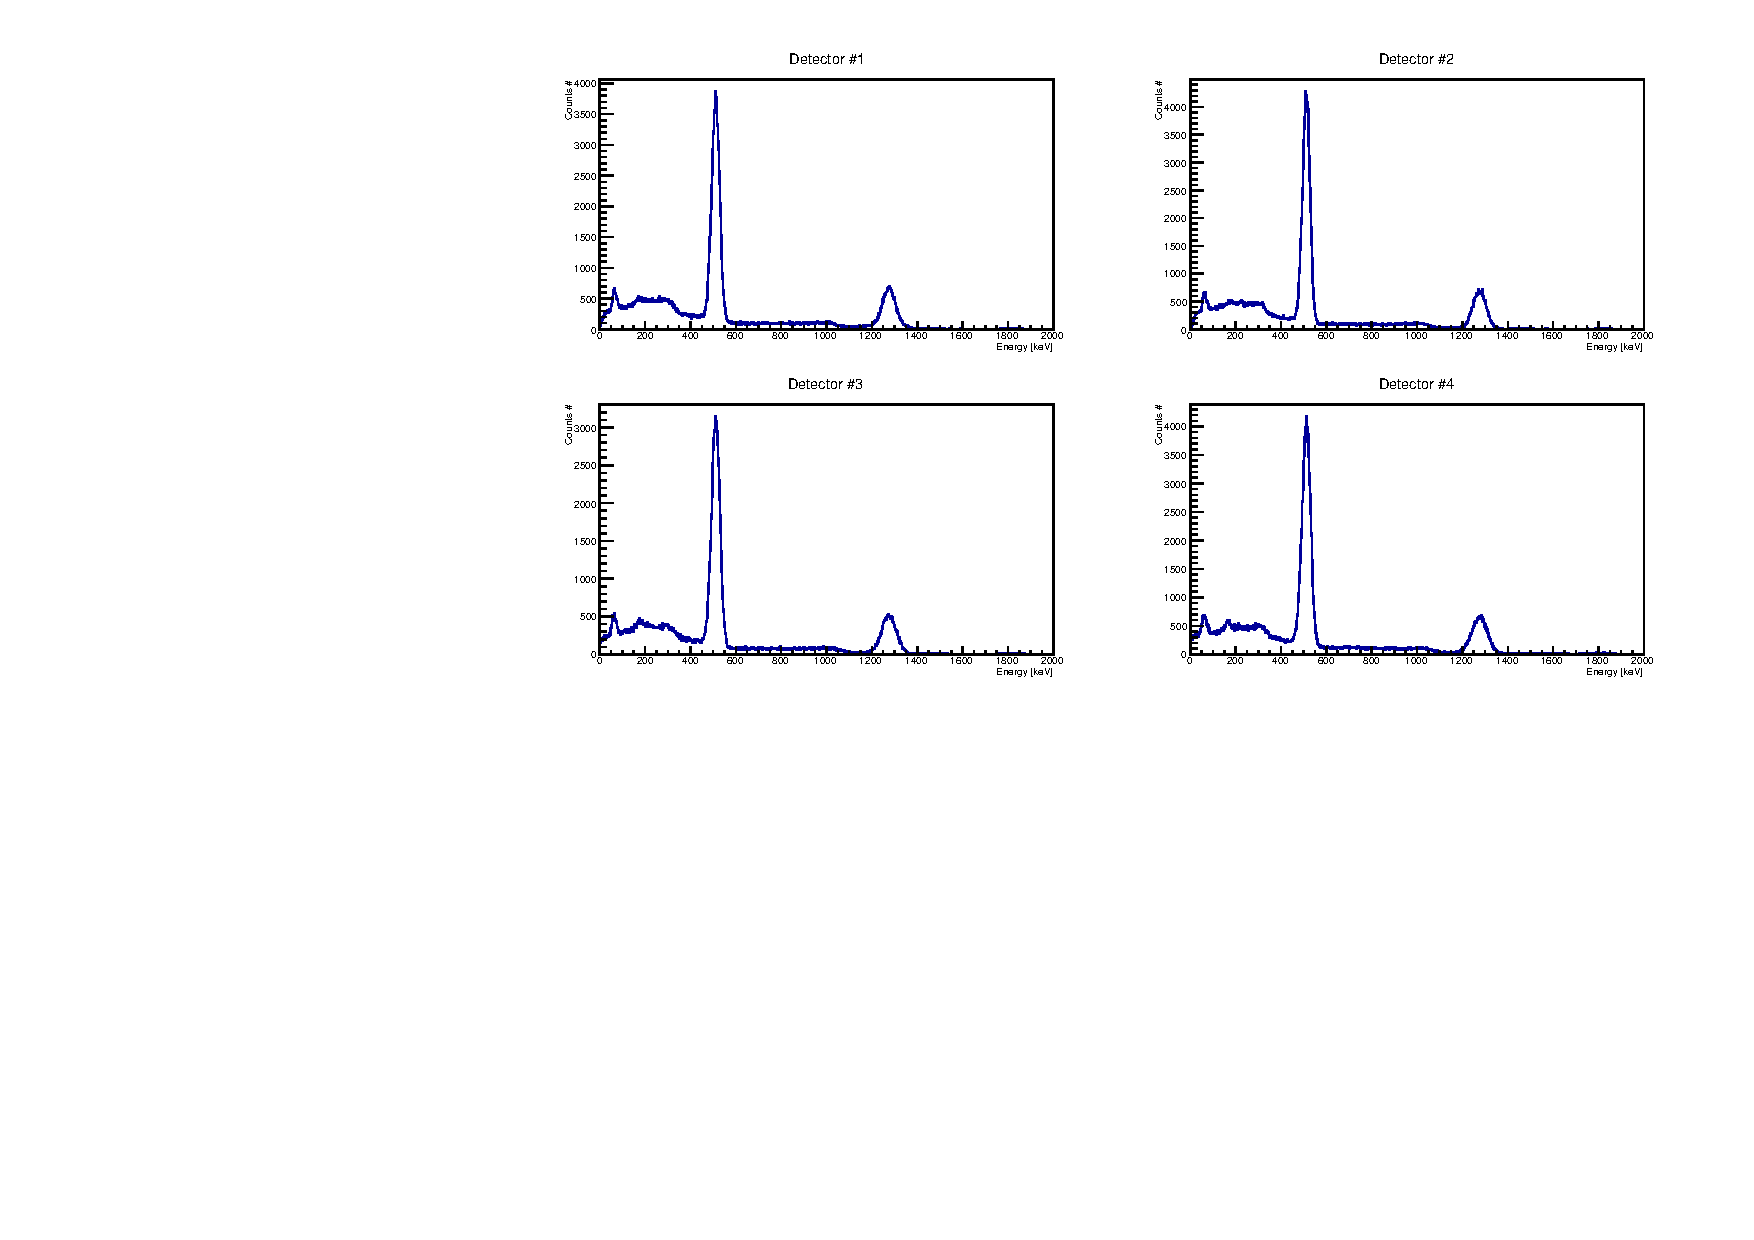
\includegraphics[width = \textwidth]{calibrated_spectra}
\caption{Calibrated $^{22}$Na energy spectra.}
\label{Fig: calibrated spectra}
\end{figure}

% Capire che errore piazzare sui parametri dei fit

\section*{TAC Calibration}

In order to calibrate the TAC unit, several spectra were produced using as start
input the CFD timing signals and as stop the same signals delayed by a chosen
value. With 2 ns delay steps the spectra of Fig.~\ref{Fig: tac calibration} was obtained, the peaks
centroids were used to compute the calibration parameters performing a linear fit (Tab.~\ref{Tab: tac calibration parameters}).

\begin{figure}[H]
\centering
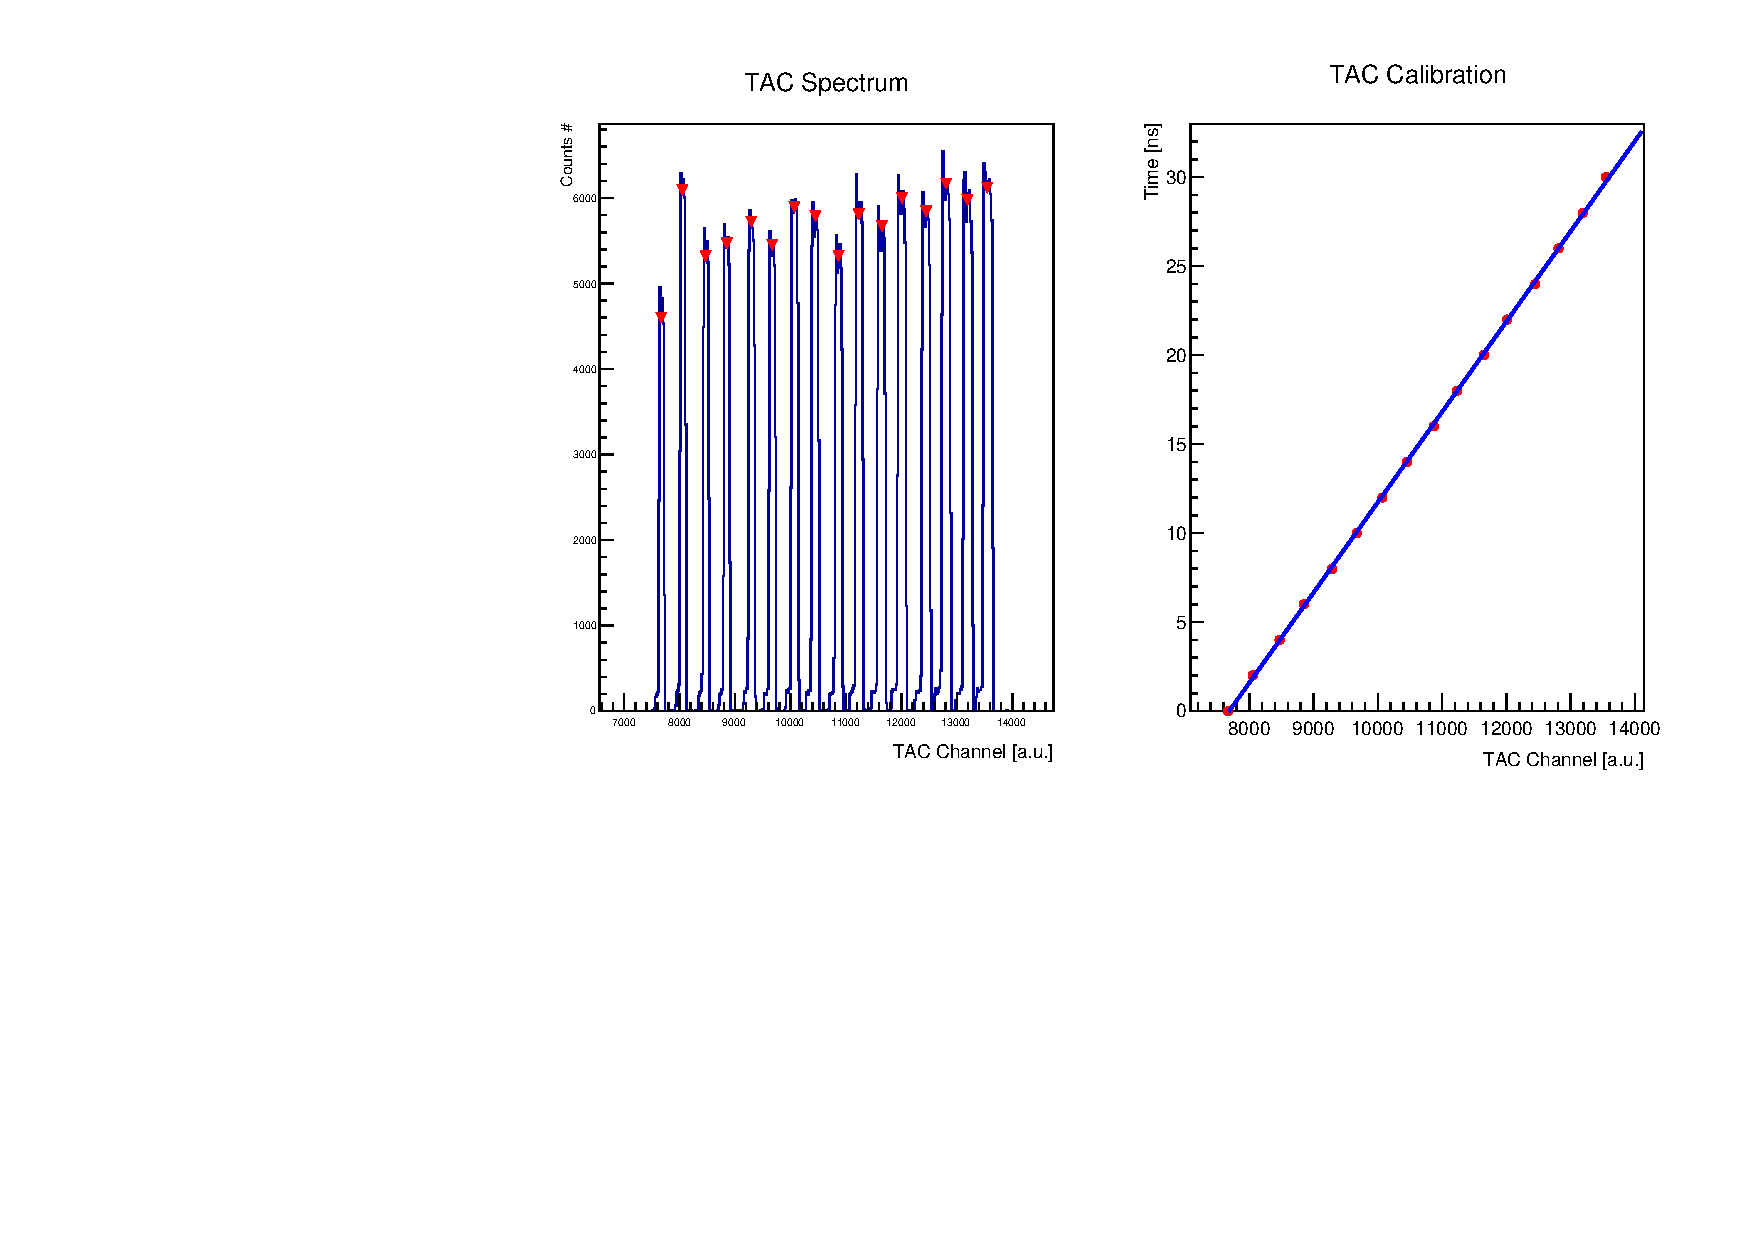
\includegraphics[width = \textwidth]{tac_cal}
\caption{TAC \textit{Auto Coincidence} spectrum and calibration Fit.}
\label{Fig: tac calibration}
\end{figure}
\begin{table}[H]
\centering
\begin{tabular}{cc}
\toprule
P0 [ns] & P1 [ns/ch] \\
\midrule
-38.9 $\pm$ 0.2 & (5.07 $\pm$ 0.02)$\times 10^{-3}$\\
\bottomrule
\end{tabular}
\caption{TAC calibration parameters.}
\label{Tab: tac calibration parameters}
\end{table}

%****************************************
%Minimizer is Linear
%Chi2                      =     0.209467
%NDf                       =           14
%p0                        =     -38.9984   +/-   0.181709    
%p1                        =   0.00507385   +/-   1.68304e-05 
